\ifx\SUM\undefined
\documentclass[journal=jacsat,manuscript=article]{achemso}

\usepackage[version=3]{mhchem}
\usepackage{booktabs}
\usepackage{float}
\usepackage{amsmath}

\newcommand*\mycommand[1]{\texttt{\emph{#1}}}

\author{Cong Wen}
\author{Xiao Tan}
\author{Wen-Hao Li}
\author{Hong-Jin Chen}
\author{Jian-Tao Zai}
%\altaffiliation{Current address: Dormitary X13 104}
\affiliation[SJTU]
	{School of Chemistry and Chemical Engineering, Shanghai Jiao Tong University, Shanghai 200240, P. R. China}
\email{zaijiantao@sjtu.edu.cn}
\phone{+86-21-34202642}

\title{An Optimization Method for Experimental Conditions of Spectrophotometric Determination of Metal Complexes}

\abbreviations{SP,phen}
\keywords{Spectrophotometric, determination of Ions, orthogonal design, Job method, molar ratio method}

\begin{document}
\fi

\section{Results and discussion}

\subsection{Find the optimization condition}
\subsubsection{Narrow wavelength range}
\begin{table}[H]
	\caption{Unifactor $\lambda$}
	\label{Tab.Uni}
	\begin{tabular}{ccc}
	\toprule
	Index	& $\lambda$/nm 	& \emph{Absorbance}\\
	\midrule
	01		& 450			& 0.305\\
	02		& 460			& 0.333\\
	03		& 470			& 0.362\\
	04		& 480			& 0.378\\
	05		& 490			& 0.385\\
	06		& 500			& 0.399\\
	07		& 510			& 0.409\\
	08		& 520			& 0.374\\
	09		& 530			& 0.292\\
	10		& 540			& 0.196\\
	11		& 550			& 0.112\\
	12		& 560			& 0.062\\
	\bottomrule
	\end{tabular}
\end{table}

\begin{figure}[H]
	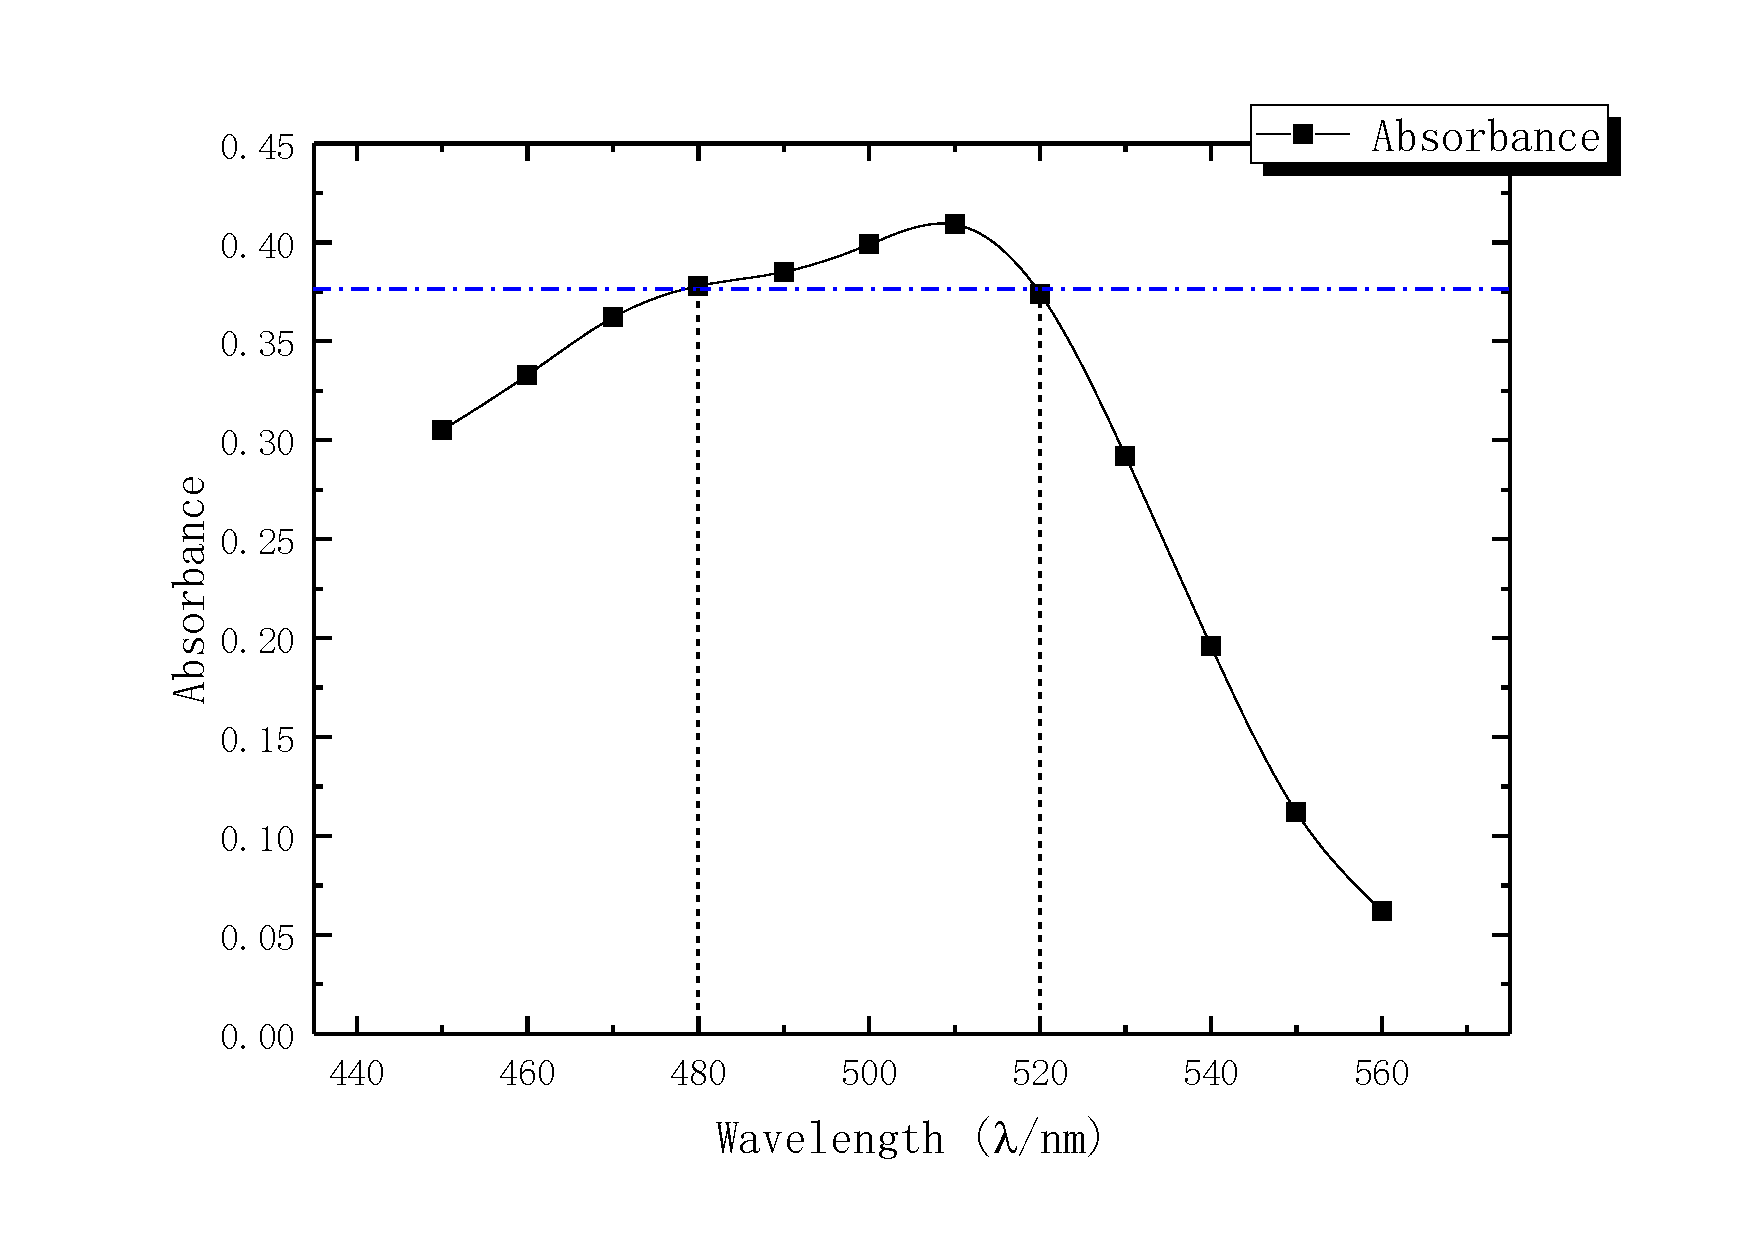
\includegraphics[width=\linewidth]{Fig0.pdf}
	\caption{Molar ratio method}
	\label{fig0}
\end{figure}

We can see intuitively from the Figure~\ref{fig0}, the wavelength corresponding to the absorbance peak must lie in $480$-$520nm$.


\subsubsection{Orthogonal experiment}
\begin{table}[H]
	\caption{Orthogonal Table}
	\label{Tab.Ort}
	\begin{tabular}{cccccccc}
	\toprule
	Index & $\lambda$/nm  & 2 &\emph{V$_{\ce{phen}}$}/mL & \emph{T}/min &\emph{V$_{\ce{NaAc}}$}/mL & 6 & \emph{Absorbance}\\
	\midrule
	01    & 488           & 1 & 0.5                & 4     & 1                  & 1 & 0.305     \\
	02    & 488           & 2 & 1                  & 6     & 3                  & 2 & 0.391     \\
	03    & 488           & 3 & 2                  & 8     & 5                  & 3 & 0.397     \\
	04    & 488           & 4 & 3                  & 10    & 7                  & 4 & 0.388     \\
	05    & 488           & 5 & 4                  & 12    & 9                  & 5 & 0.395     \\
	06    & 498           & 1 & 1                  & 8     & 7                  & 5 & 0.416     \\
	07    & 498           & 2 & 2                  & 10    & 9                  & 1 & 0.400     \\
	08    & 498           & 3 & 3                  & 12    & 1                  & 2 & 0.416     \\
	09    & 498           & 4 & 4                  & 4     & 3                  & 3 & 0.403     \\
	10    & 498           & 5 & 0.5                & 6     & 5                  & 4 & 0.319     \\
	11    & 508           & 1 & 2                  & 12    & 3                  & 4 & 0.413     \\
	12    & 508           & 2 & 3                  & 4     & 5                  & 5 & 0.433     \\
	13    & 508           & 3 & 4                  & 6     & 7                  & 1 & 0.416     \\
	14    & 508           & 4 & 0.5                & 8     & 9                  & 2 & 0.338     \\
	15    & 508           & 5 & 1                  & 10    & 1                  & 3 & 0.407     \\
	16    & 518           & 1 & 3                  & 6     & 9                  & 3 & 0.388     \\
	17    & 518           & 2 & 4                  & 8     & 1                  & 4 & 0.390     \\
	18    & 518           & 3 & 0.5                & 10    & 3                  & 5 & 0.320     \\
	19    & 518           & 4 & 1                  & 12    & 5                  & 1 & 0.392     \\
	20    & 518           & 5 & 2                  & 4     & 7                  & 2 & 0.400     \\
	21    & 528           & 1 & 4                  & 10    & 5                  & 2 & 0.305     \\
	22    & 528           & 2 & 0.5                & 12    & 7                  & 3 & 0.273     \\
	23    & 528           & 3 & 1                  & 4     & 9                  & 4 & 0.309     \\
	24    & 528           & 4 & 2                  & 6     & 1                  & 5 & 0.307     \\
	25    & 528           & 5 & 3                  & 8     & 3                  & 1 & 0.317     \\
	\bottomrule
	\end{tabular}
\end{table}

We process the data from Table~\ref{Tab.Ort} by range analysis. We use $T_i$ and $K_i$ to represent summary and average of absorbance corresponding to the $i^{th}$ level referred in Table~\ref{Tab.Fac}. The results are shown below in Table~\ref{Tab.OrtPro}.

\begin{table}[H]
	\caption{Experimental data processing}
	\label{Tab.OrtPro}
	\begin{tabular}{ccccc}
	\toprule
	& $\lambda /nm$ & $V_{\ce{phen}}/mL$ & T/min & $V_{\ce{NaAc}}/mL$\\
	\midrule
	$T_1$ & 1.876 & 1.555 & 1.850 & 1.825 \\
	$T_2$ & 1.854 & 1.915 & 1.821 & 1.844 \\
	$T_3$ & 2.007 & 1.917 & 1.858 & 1.846 \\
	$T_4$ & 1.890 & 1.942 & 1.820 & 1.893 \\
	$T_5$ & 1.511 & 1.909 & 1.889 & 1.830 \\
	$K_1$ & 0.3752 & 0.3110 & 0.3700 & 0.3650 \\
	$K_2$ & 0.3708 & 0.3830 & 0.3642 & 0.3688 \\
	$K_3$ & 0.4014 & 0.3834 & 0.3716 & 0.3692 \\
	$K_4$ & 0.3780 & 0.3884 & 0.3640 & 0.3786 \\
	$K_5$ & 0.3022 & 0.3818 & 0.3778 & 0.3660 \\
	Range & 0.0992 & 0.0774 & 0.0138 & 0.0136 \\
	\bottomrule
	\end{tabular}
\end{table}
We compare the range of each factor and draw the conclusion that wavelength and the amount of chromogenic agent have a significant impact on absorbance because their ranges are much greater, while the chromogenic time and pH have relatively weak influence. Meanwhile, Table~\ref{Tab.OrtPro} tells us the best combination of factors, on which all later absorbance measurement are based:

\begin{table}[H]
	\caption{Optimum combination of factors}
	\label{tab.Opt}
	\begin{tabular}{lcccc}
	\toprule
	& $\lambda$ & $V_{\ce{phen}}$ & T & $V_{\ce{NaAc}}$\\
	\midrule
	Optimum Index & 3(2.007) & 4(1.942) & 5(1.889) & 4(1.893)\\
	Concrete Data & 508 nm   & 3 mL     & 12 min   & 7 mL    \\
	\bottomrule
	\end{tabular}
\end{table}

\subsection{Determine composition of metal complex}

\subsubsection{Molar ratio method}

The function of fitting line on the left is $y=0.742x+0.0264(R=0.9979)$, and the function of fitting line on the right line is $y=0.254(R=1)$ which are shown below in Figure~\ref{fig2}. According to the figure, we know coordination number measured by molar ratio method is 3.07.

\begin{table}[H]
	\caption{Molar ratio method}
	\label{Tab.Mrm}
	\begin{tabular}{lcccccccc}
	\toprule
	Index         &  1  &  2  &  3  &  4  &  5  &  6  &  7  &  8  \\
	\midrule
	$V_{phen}/mL$ &1.00 &1.50 &2.00 &2.50 &3.00 &3.50 &4.00 &4.50 \\
	$V_{Fe}/mL$   &1.00 &1.00 &1.00 &1.00 &1.00 &1.00 &1.00 &1.00 \\
	$\frac{V_{phen}}{V_{Fe}}$
				  &1.00 &1.50 &2.00 &2.50 &3.00 &3.50 &4.00 &4.50 \\
	Absorbance    &0.100&0.140&0.172&0.213&0.252&0.254&0.254&0.254\\
	\bottomrule
	\end{tabular}
\end{table}

\begin{figure}[H]
	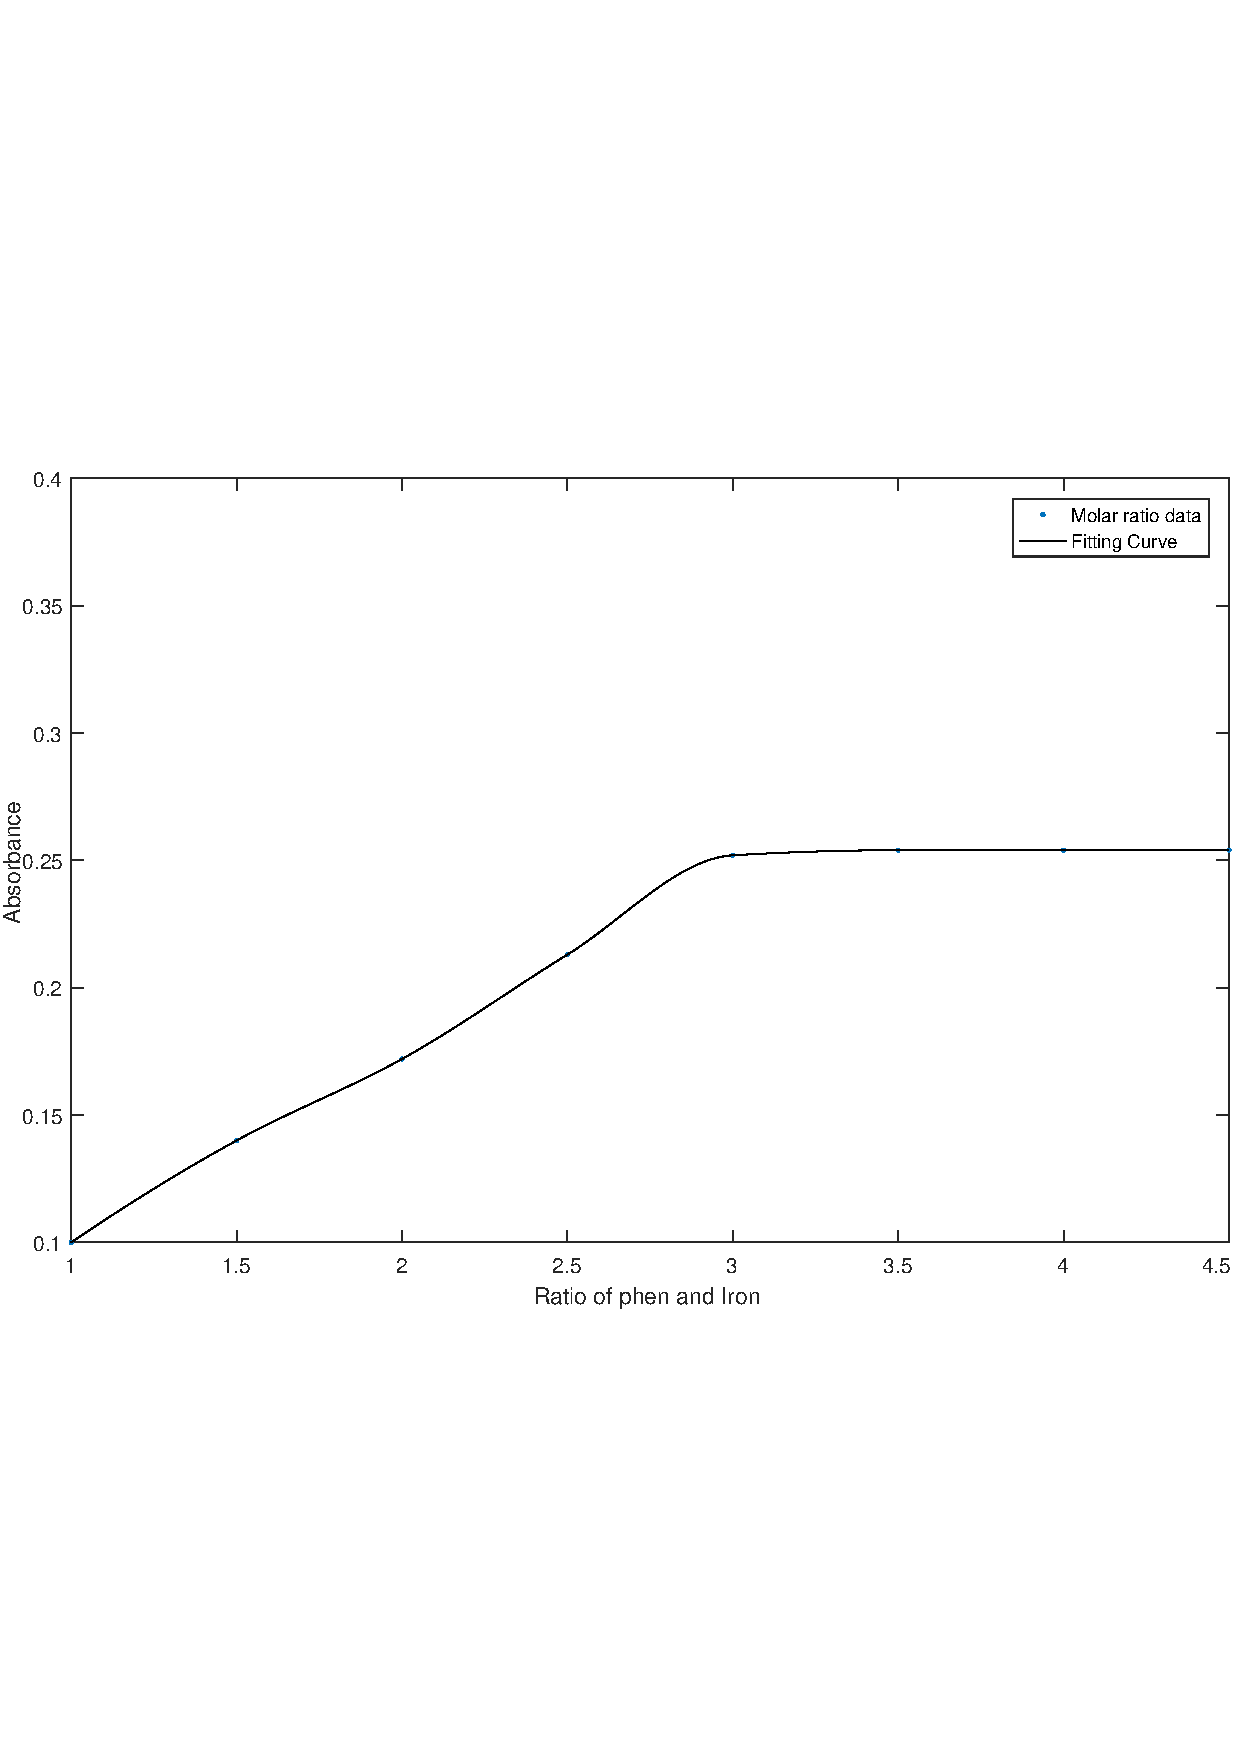
\includegraphics[width=\linewidth]{Fig2.pdf}
	\caption{Molar ratio method}
	\label{fig2}
\end{figure}

To some extent, the correlation coefficient reflects the superiority of the molar ratio method in the terms of accuracy. A reason why it is more accurate than Job method is that when $\frac{V_{phen}}{V_{Fe}}\geq3$, the slope of the line is almost 0 in theory. So compared with Job method, the molar ratio method’s correlation coefficient is closer to 1 which indicates better precision. In a word, as for studying more general coordination compound, typically whose coordination number is not 1, the molar ratio method behaves much better. According to the figure, we know coordination number measured by Job method is 2.79.

\subsubsection{By Job method}

We use $T_L$ to represent $\frac{V_{phen}}{V_{Fe}+V_{phen}}$. When $T_L<0.75$, the fitting line is $y=N/Ax-N/A(R=N/A)$, and when $T_L\geq0.75$, the fitting line is $y=-N/Ax+N/A(R=N/A)$ which are shown below in Figure~\ref{fig3}.

\begin{table}[H]
	\caption{Job method of iron}
	\label{Tab.Jbm}
	\begin{tabular}{lcccccccccccccccccc}
	\toprule
	Index
	& 1 	& 2	 	&3		& 4 	& 5 	& 6 	& 7 	& 8 	& 9 	& 10	& 11	& 12	&13		&14		&15		&16		&17		&18\\
	\midrule
	$V_{phen}$/mL
	&0.0	&1.8	&2.4	&3.0	&3.5	&4.0	&4.4	&4.8	&5.3	&5.7	&6.0	&6.2	&6.4	&6.6	&6.9	&7.2	&7.5	&8.0\\
	$V_{\ce{Fe}}$/mL
	&8.0	&6.2	&5.6	&5.0	&4.5	&4.0	&3.6	&3.2	&2.7	&2.3	&2.0	&1.8	&1.6	&1.4	&1.1	&0.8	&0.5	&0.0\\
	$T_L$
	& 0.00 	&0.23	&0.30	&0.38	&0.44	&0.50	&0.55	&0.60	&0.67	&0.71	&0.75	&0.78	&0.80	&0.83	&0.86	&0.90	&0.94	&1.00\\
	$Absorbance$
	&   	&0.141	&0.185	&0.252	&0.252	&0.330	&0.377	&0.410	&0.441	&0.490	&0.490	&0.405	&0.368	&0.340	&0.258	&0.186	&0.117	&\\
	\bottomrule
	\end{tabular}
\end{table}

\begin{figure}[H]
	\includegraphics[width=\linewidth]{Fig3.pdf}
	\caption{Job method of iron}
	\label{fig3}
\end{figure}

The reason why the measured coordination number is smaller than theoretical number is when $T_L\geq3.0$, we only use four points to fit the line, and less points means less accuracy, which is unavoidable when the coordination number isn't $1$. Besides, the slope of the theoretical line on the right is so great, which indicates a large relative deviation. Specifically, let's see the results of determining composition of copper(\uppercase\expandafter{\romannumeral2}) and sulfosalicyclic acid complex using Job method.

We use $T_L$ to represent $\frac{V_{\ce{H3SSR}}}{V_{\ce{Cu(NO3)2}}+V_{\ce{H3SSR}}}$. When $T_L<0.5$, the fitting line is $y=N/Ax-N/A(R=N/A)$, and when $T_L\geq0.5$, the fitting line is $y=N/Ax+N/A(R=N/A)$ which are shown below in Figure~\ref{fig4}.

\begin{table}[H]
	\caption{Job method of copper}
	\label{Tab.Jbm2}
	\begin{tabular}{lccccccccccccc}
	\toprule
	Index					&1		&2		&3		&4		&5		&6		&7		&8		&9		&10		&11		&12		&13\\
	\midrule
	$V_{\ce{H3SSR}}$/mL 	&0		&2		&4		&6		&8		&10		&12		&14		&16		&18		&20		&22		&24\\
	$V_{\ce{Cu(NO3)2}}$/mL  &24		&22		&20		&18		&16		&14		&12		&10		&8		&6		&4		&2		&0	\\
	$T_L$					&0		&0.083	&0.167	&0.250	&0.333	&0.417	&0.500	&0.583	&0.667	&0.750	&0.833	&0.917	&1.000\\
	$Absorbance$ 			&0.037	&0.076	&0.140	&0.245	&0.274	&0.296	&0.312	&0.310	&0.298	&0.244	&0.171	&0.097	&0.031\\
	\bottomrule
	\end{tabular}
\end{table}

\begin{figure}[H]
	\includegraphics[width=\linewidth]{Fig4.pdf}
	\caption{Job method of copper}
	\label{fig4}
\end{figure}

It's very clear that if the coordination number is $1$, the position of absorbance peak is easy to tell and the line on the two sides are fitted more accurately with less point. So molar ratio method is always available in principle, while as for complexes with large coordination number, such as \ce{[Fe(CN)6]}$^{3-}$, it's reasonable to predict that the absorbance peak will be pushed aside along with the axis, which is really difficult for us to tell it's accurate composition.


\subsection{Purity measurement of \ce{FeC2O4}$\cdot$2\ce{H2O}}

\subsubsection{Spectrophotometric method}

\paragraph{Plot standard curve}
Using data from Table~\ref{tab.Cal}, we plot the standard curve which is shown in Figure~\ref{fig1}, the function of fittineline is $y=0.2026x+0.00076(R=0.9995)$, so it is reasonable to think it pass the origin accurately. Then we can use this curve to determine the concentration of iron in unknown sample as long as we dissolve it and measure its absorbance.
\begin{table}[H]
	\caption{standard curve data}
	\label{tab.Cal}
	\begin{tabular}{lllllll}
	\toprule
	$V_{Fe}$/mL    & 0.0 & 1.0 & 2.0 & 3.0 & 4.0 & 5.0 \\
	$c_{Fe}/\mu$g$\cdot$mL$^{-1}$
				   & 0.0 & 0.4 & 0.8 & 1.2 & 1.6 & 2.0 \\
	\midrule
	$Absorbance$     &0.000&0.081&0.166&0.247&0.316&0.410\\
	\bottomrule
	\end{tabular}
\end{table}

\begin{figure}[H]
	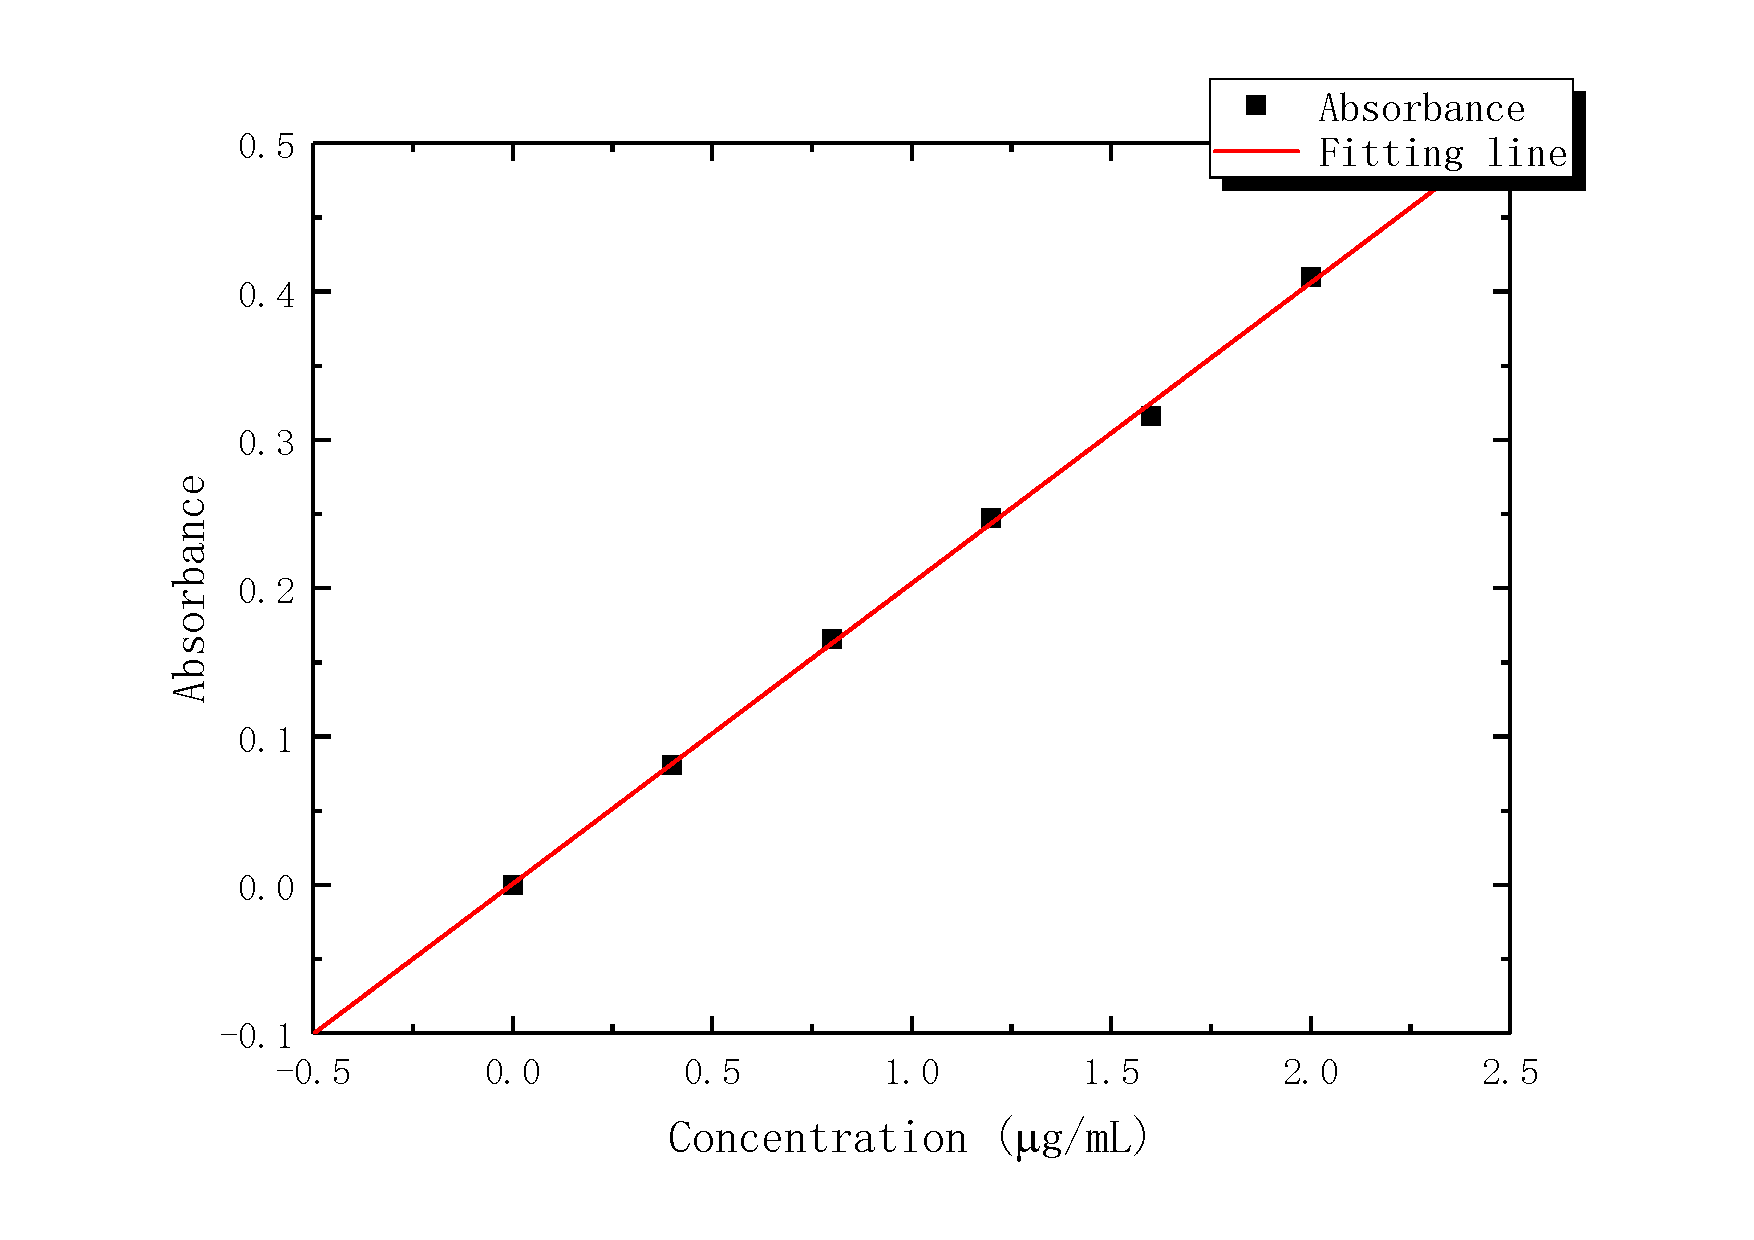
\includegraphics[width=\linewidth]{Fig1.pdf}
	\caption{standard curve}
	\label{fig1}
\end{figure}

\paragraph{Concentration determination}
We apply the standard curve to determine the concentration of iron in our self-made \ce{FeC2O4}$\cdot$2\ce{H2O} sample, therefore getting purity easily by simply calculating: \[\omega=\frac{c_{Fe}\times250{\rm mL}\times179.9{\rm g/mol}}{m_{sample}}\].

\begin{table}[H]
	\caption{Purity Measurement by standard curve}
	\label{tab.Pcurve}
	\begin{tabular}{ccccc}
	\toprule
	Sample Index  &$Mass$/g & $Absorbance$ &$c_{Fe}/\mu$g$\cdot$mL$^{-1}$& $purity$   \\
	\midrule
	1		&0.2083 & 0.546      & 2.52   &$97.2\%$  \\
	2		&0.2170 & 0.534      & 2.46   &$91.1\%$  \\
	3		&0.2023 & 0.501      & 2.31   &$91.8\%$  \\
	4		&0.2020 & 0.509      & 2.35   &$93.5\%$  \\
	5		&0.2048 & 0.517      & 2.38   &$93.4\%$  \\
	6		&0.2184 & 0.530      & 2.44   &$89.8\%$  \\
	\bottomrule
	\end{tabular}
\end{table}

\subsubsection{By titration method}

We can first get the concentration of standard potassium permanganate solution easily using data from Table~\ref{tab.CalMn} by calculating: \[c_{\ce{KMnO4}}=\frac{2}{5}\times\frac{m_{\ce{NaC2O4}}}{134.0{\rm g/mol}\times V_{0average}}=0.01895{\rm mol/L}\].

\begin{table}[H]
	\caption{standard of \ce{KMnO4}}
	\label{tab.CalMn}
	\begin{tabular}{ccc}
	\toprule
	Index\textsuperscript{\emph{a}}&$V_0$/mL&$V_{0average}$mL\\
	\midrule
	1    & 24.44 &\\
	2    & 24.42 & 24.43\\
	3    & 24.42 &\\
	\bottomrule
	\end{tabular}\\
	\textsuperscript{\emph{a}}:Mass of sample \ce{NaC2O4}=$6.2013$g
\end{table}

\begin{table}[H]
	\caption{Titration of \ce{FeC2O4}$\cdot$2\ce{H2O}}
	\label{tab.Tit}
	\begin{tabular}{ccccccc}
	\toprule
	Index\textsuperscript{\emph{a}}&$V_{1start}$/mL&$V_{1end}$/mL&$V_{1average}$/mL&$V_{2start}$/mL& $V_{2end}$/mL&$V_{2average}$/mL\\
	\midrule
	1    & 0.10 & 30.60 &       & 0.00 & 9.85 &     \\
	2    & 0.00 & 30.48 & 30.49 & 0.00 & 9.90 & 9.85\\
	3    & 0.00 & 30.50 &       & 0 00 & 9.80 &     \\
	\bottomrule
	\end{tabular}\\
	\textsuperscript{\emph{a}}:Mass of sample \ce{FeC2O4}$\cdot$2\ce{H2O} =$1.8012$g;
\end{table}

Then we can easily calculate the purity by calculating: \[\omega=\frac{5}{2}\times\frac{V_{2average}\times c_{\ce{KMnO4}}\times179.9{\rm g/mol}}{m_{sample}}\times\frac{250{\rm mL}}{25{\rm mL}}=93.2\%\]


\subsubsection{Accuracy comparision}
The comparision of purity measured betweem titration method and spectrophotometry is shown in Table~\ref{tab.Res}.

\begin{table}[H]
	\caption{Purity comparision}
	\label{tab.Res}
	\begin{tabular}{ccc}
	\toprule
		   & Titration & standard\\
	\midrule
	Purity & $93.2\%$  & $93.4\%$\\
	\bottomrule
	\end{tabular}
\end{table}

We find the result of using standard curve is in comformity with that of using titration method, therefore validating the accuracy of spectrophotometry and illustrating that spectrophotometry really meets the requirement of green chemistry.

\ifx\SUM\undefined
\bibliography{reference}
\end{document}
\fi